%!TEX root = ../thesis.tex

\cleardoublepage
\chapter{Background}
%\chapter{Background Information and Related Work}
\label{cha:background}

To place this thesis in its proper academic and practical context, this chapter will provide background information on relevant topics as well as reviewing some of the literature which bears similarity or served as an inspiration. First, mobile networking and 5G will be covered, then multipath solutions, and finally deterministic networking.

\section{Mobile Networks and Backhaul}

For the sake of brevity, the full history of the development of mobile networks will be hugely condensed and simplified, and only the 5G architecture will be explained in depth.

The defining characteristic of a mobile network is wireless connectivity. This enables the users to move around while remaining connected to the network, which stands in direct opposition to historical computer networks which were stationary and usually featured fixed connections between computers. A user in a mobile network must first detect and then connect to a Base Station, this process includes authentication and authorization. A user may be switched from one Base Station to another depending on the signal strength (this is referred to as a handover), and this is what enables the user to maintain a connection whilst moving across wide areas. In mobile networks which support IP traffic, the user will normally appear to remain behind a single IP address despite their mobility.

All of the user's data sent to the network goes through the Base Station to which it is currently connected. At first this data was exclusively analog voice data, however over time newer versions of the mobile networking specifications have defined different types of data, and eventually defined support for Internet Protocol (IP) messages as well. Starting with 4G, mobile networks transitioned to an all IP architecture \cite{3gpp.36.300}. To support and manage user mobility and provide internet connectivity, today's mobile networks have a complex core network architecture where different Network Functions (NF's) are responsible for the different aspects of user management. This core network continues to evolve with each new specification.

\begin{figure}[ht]
    \centering
	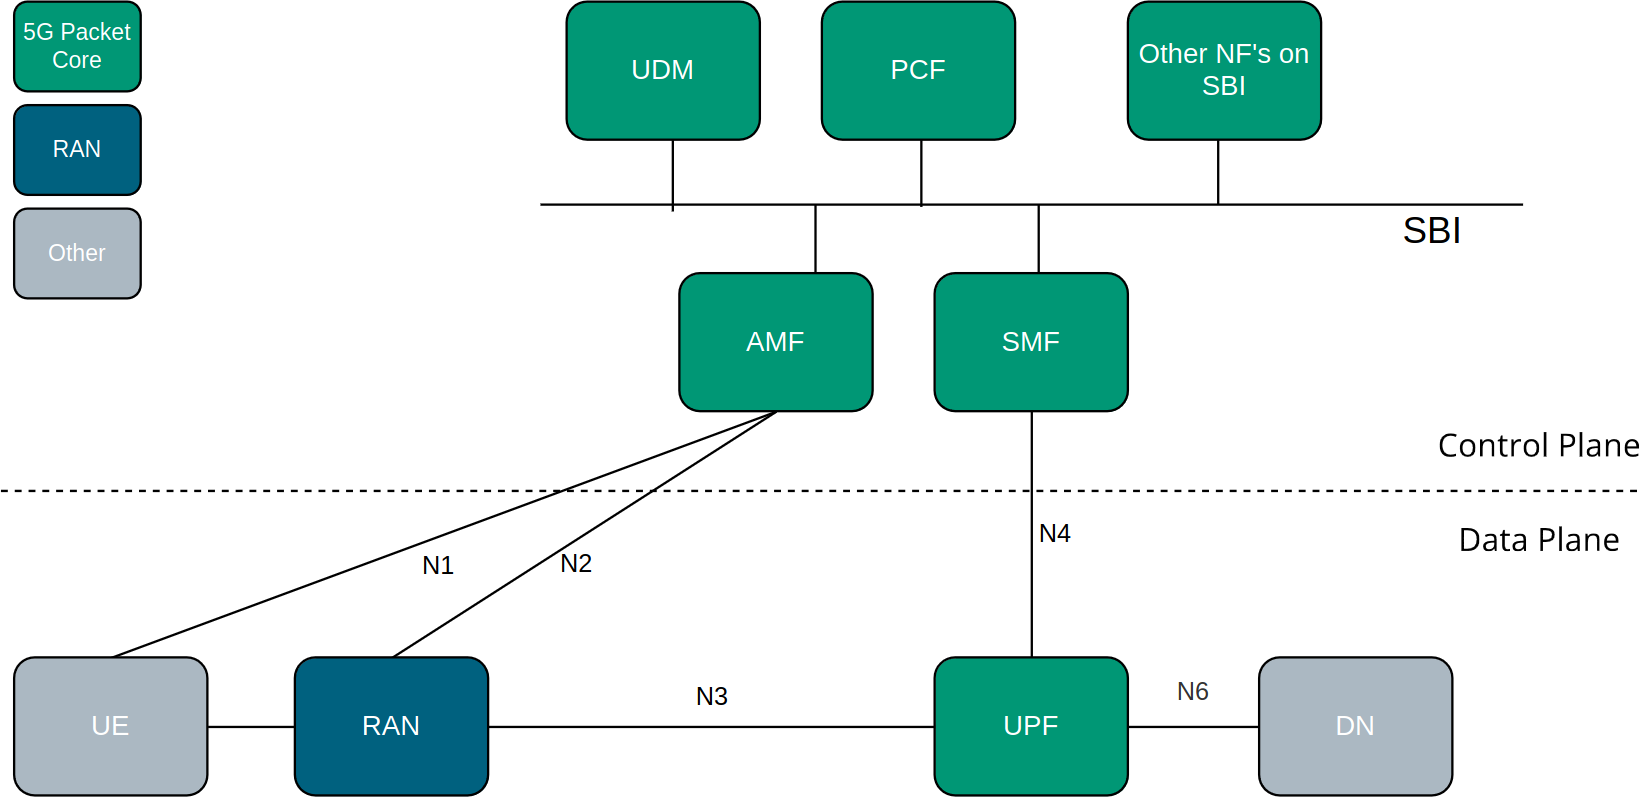
\includegraphics[width=\linewidth]{fig/core.png}
	\caption{Simplified 5G Architecture}
	\label{fig:core}
\end{figure} 

Figure \ref{fig:core} shows a simplified version of the architecture of a 5G core network and how it is connects to the RAN, the user, and the internet. The figure does not include all of the Network Functions defined in the 5G specifications but shows a select few which will be briefly explained in following.

The Access and Mobility Management Function (\textbf{AMF}) handles, among other things, the user registration (access authentication and authorization), connectivity management, and the control plane interface to the RAN. The reference point for interactions between the AMF and the RAN is called the N2 reference point. The reference point for interactions with the UE is N1. This is a purely logical interface, messages between the UE and the AMF actually have to physically go through the RAN.

The User Plane Function (\textbf{UPF}) is responsible for forwarding packets between the Data Network and the RAN. The UPF must also perform QoS enforcement, for example making sure users do not exceed the bandwidth limits of their subscription. The UPF communicates with the RAN over the N3 reference point. For this they utilize the GPRS Tunneling Protocol (GTP). GTP is a tunneling protocol designed for mobile networks. Packets originating in the RAN are contained in a GTP tunnel and must be de-capsulated by the UPF before being forwarded to the Data Network (DN). Packets in the opposite direction must have a GTP header added to them before they are sent to the RAN.

The Session Management Function (\textbf{SMF}) is responsible for session establishment and management, and it configures traffic steering in the UPF. The SMF and the UPF communicate over the Packet Forwarding Control Protocol (PFCP) on the N4 reference point. Their interactions are a lot like those between a switch and a controller in a Software Defined Network (SDN), with the SMF acting as the controller.

The Policy Control Function (\textbf{PCF}) provides policy rules to different Control Plane functions in order to enforce them. The SMF consults the PCF before informing the UPF what Quality of Service a given user should experience. The interactions between the SMF and the PCF go over the Service Based Interface (SBI). This is a logical interface which represents all of the different interactions between all of the Control Plane Network Functions. All communication on the SBI uses HTTP2.

In the figure it can also be seen how the 5G Core (like the 4G Packet Core before it) splits the control plane and the user plane (or data plane). The network functions in the control plane co-ordinate to make decisions over how to orchestrate the user plane, while the components in the data plane are the ones forwarding the actual user traffic.

\subsection{5G and Campus Networks}

In order to enable new industrial use cases, 5G campus networks may be deployed exclusively for users within a campus organization, and covering only a prescribed geographical area \cite{rischke20215g}. The deployment of such a network can be crucial for time-sensitive wireless communication, e.g. between robots, and the 5G specifications contain traffic classes and QoS requirements for delay-critical use cases \cite{3gpp.23.501}. This is done in order to make 5G a competitive, or even superior, option to WiFi in campus deployments \cite{walia20175g}.

There is lots of room for different deployment architectures for 5G campus and non-public networks (NPN's). In \cite{prados20215g} many of these architectures are discussed and investigated. In order to operate a 5G campus network, spectrum may need to be acquired, as well as 4G or 5G base stations, depending on the mode of operation- NSA (non-standalone: 4G Base Stations (eNodeB's) but a 5G Core Network) or SA (standalone: 5G Base Stations (gNB's) and a 5G Core Network). Furthermore, a 5G Core Network is required in order to manage the network. Since 5G places an increased focus on virtualization and flexibility of deployment, there are a litany of options for which network functions from the core to deploy, and where to deploy them.

This thesis addresses specifically those campus network deployments which require backhaul to a core located off premises. Networks deployed in this fashion will typically feature a subset of the core's network functions deployed on premise. In the simplest case the only component on premise will be the RAN. A different deployment model may feature one UPF on site with a second UPF located in the core, and the backhaul takes place between the two UPF's. This thesis' WAN Connector will be designed to be able to backhaul IP traffic from the remote campus to the core, either between the RAN and the UPF, or between two UPF's.


\subsection{Backhaul in 5G}

The first hop from the user equipment (UE) into the mobile network occurs over the air, via wireless signals. This communication is between the UE and the Base Station. The network of different Base Stations is called the Radio Access Network (RAN). Once the user has transmitted its data to the RAN, the RAN is responsible for passing on the user's messages to the core network. The transport network between the RAN and the Core is the backhaul network, or “backbone" \cite{jaber20165g}. However the term backhaul can also be used to refer to the process of transporting data from the RAN back to the core.

In light of the increased focus in 5G on enabling time sensitive industrial use cases, the authors in \cite{prados2021asynchronous} proposed a method for integrating asynchronous Time Sensitive Networking (TSN) into 5G backhauling. To achieve this their architecture uses an Asynchronous Traffic Shaper, which is crucial for integrating the time sensitive traffic with the regular traffic. Their solution also utilized frame replication for the delay critical flows defined in the 5G specifications (5G QoS Identifiers (5QIs) 82 through 85).

The authors of \cite{jaber20165g} highlight the need for innovation in 5G backhaul provisioning. At present optic fibre backhaul is not available nationwide in Europe, and Fibre to the Home (FTTH) is scarce worldwide. Currently most backhaul networks are built with microwave links or fibre/copper based links. There has also been research \cite{seppanen2016multipath, saadat2018multipath} into using multipath routing within the context of millimeter Wave (mmWave) backhaul in order to increase both reliability and throughput.

Another option for mobile backhaul is satellite constellation networks. Geostationary Orbit satellites (GEO satellites) appear motionless to observers from the ground, and thus provide consistent latency and jitter. However this comes at a cost, they are a large distance away from the earth and round trip times are routinely on the order of 400 to 500 milliseconds. Regardless, GEO satellites are still a crucial means for connectivity for remote regions and areas where it is not possible or very difficult to provide other means of backhaul. Recently, Low-Earth Orbit (LEO) satellite constellations have begun to emerge and represent a more appealing option due to their greatly reduced latencies when compared with GEO satellites \cite{deutschmann2022broadband}. The 3G Public Partnership Project (3GPP), who are behind the 5G specifications, have commissioned a technical report, TR 23.737 \cite{3gpp.23.737}, on possible architectures and integration scenarios for satellite backhaul in 5G. Furthermore, independent studies have also highlighted the usefulness of satellite backhaul for 5G, and identified it as a key enabler of some of the goals set for 5G \cite{artiga2016terrestrial}.

In light of the increased focus on using satellite backhaul, the technical report mentioned above identifies one scenario which pertains exactly to this thesis. The “key issue \#9" in the report: “multi connectivity with hybrid satellite/terrestrial backhaul". The report constructs a specific use case for hybrid backhaul. Consider Additive Layer Manufacturing (ALM) factories, wherein the command and monitoring systems for the automation of the factory require reactivity, and machines in the factory must download the ALM electronic files. This download process will saturate the network resources and requires high bandwidth, conversely the automation processes will need low latency and low bandwidth. In order to meet the different requirements of the two applications, the file transfer could be sent over the satellite backhaul, while the remote command and monitoring could take place over the terrestrial link. Precisely this kind of situation highlights the need for a deterministic multipath backhaul solution for 5G campus networks. Here, this thesis addresses the issue more generally, aiming to develop a system that can handle more backhaul options than just one terrestrial link and one satellite link.


\section{Multipathing and Multihoming}

At this point it becomes important to establish the definitions of two similar terms, and how they will be used in this thesis. Multihoming refers to a host, organization, or network, having more than one external link- either to the same Internet Service Provider (ISP), or to more than one \cite{akella2003measurement}. A multihomed host can choose to use different links for different traffic. Multipath routing, on the other hand, is a routing approach which selects separate paths when routing packets. In order to perform multipath routing there must be more than one path from the source to the destination, and the source must be able to choose which path to take. If the source or destination or both are multihomed then it is possible to choose from more than one path between the two of them. In this thesis the term multipathing will be used interchangeably with multipath routing.

This discussion ties into the difference between links (or interfaces) and paths. When two multihomed hosts are communicating, using the same outgoing link does not mean taking the same path. The same interface could be used to send packets with different destination IP addresses and then the packets would take different paths. It is only in the context of a multihomed host communicating with a host that only has one IP address, that selecting a different interface is the same as selecting a different path. In these cases alone, multihoming and multipathing are the same.

With these definitions in hand, we will now review some of the existing literature to see what kinds of approaches have been taken to address problems similar to those of this thesis.

\subsection{Collecting and/or Predicting Performance Metrics in a Multihomed Environment}

In \cite{akella2008performance} the authors collected both passive metrics (looking at response times for outgoing packets), and active measurements (sending ICMP ping, or TCP SYN messages and measuring the response time). Using the passive measurements enabled their multihomed approach to perform well, but when using the active measurements the performance was even better. Crucially, the passive measurements worked better over larger sampling periods, because it took longer to get a full overview of all the possible routes, whereas the active sampling approach acquired it's measurements faster and was thus more effective over smaller sampling intervals.

Considering this result, the solution developed in this work will therefore utilize forms of both active and passive measurements. All three metrics- packet loss, latency, and jitter- will be periodically measured in an active manner. The period over which to perform these measurements is also an important design decision for the WAN connector, and it will be a fixed value, which can be configured by the operator. The use of a fixed value is important in the context of a solution which aims to provide determinism, since traffic may often have hard requirements for the maximum tolerable latency, packet loss, or jitter, which a flow is allowed to experience within a given window. For example in the 5G QoS specifications the averaging window for non delay critical traffic is 2 seconds \cite{3gpp.23.501}.

For classical wired links in multihomed scenarios, \cite{tao2004exploring} have observed that one link will generally dominate with regards to latency, but with brief periods where other links' performance is superior. These same authors also note that with regards to packet loss there is far less prevalence of a “dominant" link, and generally the links will perform comparably. Packet loss is also a particularly difficult metric to measure, since most links are highly reliable and when they do experience packet loss it is in bursts \cite{tao2004exploring}. Wireless connections are usually less reliable and may experience more consistent rates of packet loss at the data link layer, however often this is opaque from the perspective of the higher layers and hard to perceive.

Ultimately, many of the best performing approaches for predicting packet loss, e.g. Hidden Markov Models \cite{tao2004exploring, bremler2002predicting}, are still somewhat imprecise and inaccurate. These models assume the link is in one of two states, good or bad, and each state has a different probability for packet loss, and there is a transition matrix which represents the probabilities of switching from one state to another.

\subsection{Path and/or Interface Selection}

Multipath routing approaches, as well as interface selection in multi-homed environments are mature and well researched topics. Here, a selection of such approaches is covered.

Wireless Sensor Networks (WSN's) are often deployed in challenging environments and must construct their routing tables dynamically. Research into multipath routing solutions for providing QoS guarantees in WSN's can serve as inspiration for this thesis' approach. In  \cite{huang2008multiconstrained}, the authors address QoS provisioning in a WSN, using multipath routing. Their approach is to formulate the problem as a probabilistic programming problem and then convert it to a linear programming problem using an approximation technique. When solved, the equation they use to represent the problem yields which paths packets should be sent on (or duplicated on) in order to achieve the desired reliability. Only those paths which would guarantee the maximum latency is still below the QoS requirements are considered. This approach bears similarity to how \cite{prados2021asynchronous} (discussed earlier) uses frame replication for certain flows.

Another article which deserves mentioning is the work in \cite{akella2008performance}. Here, the authors evaluate a large set of route-control mechanisms and evaluate their trade-offs for multihomed enterprises, in order to derive “best common practices" for multihoming. Their most important results shows that there is no benefit to using historical samples; route selection should always be based on current samples. They even find that employing historical data to make decisions about which path to forward on can prove detrimental at times.

We may also look at the work in \cite{habib2007improving}, where the authors investigate the use of residential multihoming to improve QoS. Their work suggests that even the use of a rudimentary switching algorithm is enough to improve QoS by switching the outgoing ISP based on \textit{any} metric. The authors observed that most of the time, the decision to switch ISP's based on one metric is consistent with the decision that would be made by considering the other metrics.

In the context of improving QoS we can see that \cite{tao2005improving} also used a simple path switching algorithm and were able to get positive results. They dynamically adapt the time scale over which these path switching decisions are made by tracking the improvement that would have been possible for each possible value $t$ among a set of predefined options $\{t_n;n = 1,2, ... N\}$, and changing $t$ if there is a $t_n$ that gives enough of an improvement. By maintaining an exponentially weighted moving average, they give higher weight to the most recent measurements and the corresponding theoretical improvements that would have been possible for different values of $t$.

Lastly, we can look to the work in \cite{goldenberg2004optimizing}, which also addresses the issue of cost in it's approach. It presents several different algorithms, including one which minimizes cost by ensuring no ISP serves more traffic than its charging volume is proportional to (e.g. only serve 95th percentile charging volume 5\% of the time). It also presents both an offline approach which solves a Mixed Integer Programming problem, and an online approach which performs greedy assignment by always switching to the ISP with the best predicted performance, out of all the ISP's able to provide the required capacity.

%Finally the last work which will be discussed is \ref{rodriguez2004mar}. In this work, the authors built a commuter mobile access router infrastructure which uses multiple wireless service providers. Much like the WSN examples this approach is a wireless multihomed device.

\section{Determinism in Computer Networking}

%\subsection{Quality of Service (QoS)}

\subsection{Deterministic Networking Specification}

Whilst TSN is able to provide the desired reliability and timing that critical applications require, there is a need for this sort of support in networks which are too large to be classified as Local Area Networks (LANs) \cite{detnet-use-cases, detnet-problem-statement}. To this extent, Deterministic Networking aims to enable the migration of applications suited for TSN's to larger packet switched networks, while maintaining support for existing packet network applications over the same physical network \cite{detnet-problem-statement}.

In this thesis, “determinism" does not refer to the IETF DetNet Working Group's definition. However it is still important to consider their specifications and their definition of a Deterministic Network (DetNet), from which our own definition of deterministic backhaul can be built.

The Deterministic Networking Problem Statement contains certain requirements of the network as a whole. These are not possible for this thesis, which addresses backhaul over resources which are not controlled by the operator. The WAN Connector, once implemented, will only be able to select from the available backhaul connections, it has no control over their network. Beyond this however, the problem statement's definition of determinism can be used. This entails absolute guarantees of minimum and maximum latency as well as packet loss and jitter, and secondly the use of more than half of the network's bandwidth. The latter is a crucial aspect of the definition since it prohibits massive over-provisioning of resources, which is an inefficient solution.

\subsection{Traffic Shaping, Fair Queuing, and Bufferbloat}

The DetNet Architecture specification \cite{detnet-arch} explicitly mentions the use of a traffic shaper to avoid contention loss, but also warns against causing bufferbloat by using oversized buffers while trying to prevent contention loss. This subsection explores what these are and what they entail.

First, to bufferbloat; this phenomenon refers to the use of disproportionately sized buffers, and their effect on the latencies experienced when these buffers are full \cite{allman2012comments, gettys2011bufferbloat}. The TCP congestion avoidance algorithm depends on dropped packets in order to detect when the bottleneck link along the path is saturated, and reduce its window size in response. When congested links finally do drop packets, if these packets are the last ones in the queue it means the whole rest of the queue must be sent first before the dropped packets are detected and the window size is reduced. This means that there is an unnatural delay before congestion is detected, and during that period all packets passing through the node experience unnecessary latency. %This problem has been heavily exacerbated by the cheap availability of memory and the desire for low packet loss. This is a fundamental misunderstanding. Dropping TCP packets is a means of communication and is not at all the same as packet loss which occurs to equipment failure or transmission errors. By dropping packets when a TCP flow exceeds its throughput, congestion is communicated. This problem can occur with UDP as well but it is even harder to detect in those instances.

The first solution to this problem lies in properly sized buffers, another solution is Early Congestion Notification (ECN), wherein TCP is explicitly warned of congestion through flags in the IP headers of messages going back to the sender, instead of through dropped packets. The other solution comes in the form of traffic shaping. Specifically, by using active queue management and fair queuing, respectively,  it is possible to selectively drop packets from a buffer (e.g. only those for a greedy TCP flow) and dequeue other packets earlier (e.g. a different flow which is not congesting the link). This overcomes the bufferbloat problem by causing the greedy TCP flow to reduce its throughput and letting through those flows that are not using more than their share of the bandwidth.

Beyond mitigating bufferbloat, traffic shaping can still be crucial for latency sensitive applications. Contention loss and queuing delays can be avoided by smoothing out any large bursts of packets. Furthermore, which traffic shaper to use is a fundamental design decision that must be made. If a link is kept busy at all times, so that maximum throughput is achieved, it means that latency critical packets may not always be forwarded on time. Conversely, by reserving some portion of the bandwidth in case latency sensitive traffic arrives, the full bandwidth cannot be used at all times and thus the throughput is reduced. This is a fundamental trade-off which cannot be avoided.

%A traffic shaper is also important for reducing packet loss. In packet switched networks the only source of packet loss which does not arise from a lower layer is when packets are dropped due to buffers overflowing. This occurs naturally in networks with “bursty" traffic because the natural distribution of bursts of packets mean that occasionally there will be overlapping bursts of packets which cause a link to become congested and drop packets. This is where traffic shaping and queue management is crucial. The bursts may be smoothed out before the bottleneck link, by releasing packets at a slower rate or dropping those that can afford being dropped (if there are any!). It should be noted that a similar effect can also be achieved through resource reservation and/or through a scheduler which makes sure to never over-schedule the network's resources. However this requires exact knowledge of the maximum bandwidth requirements of all the packet flows in the network.


A traffic shaper is also important for reducing packet loss. By releasing packets at a slower rate or dropping those that can afford to be dropped, bursts of packets may be smoothed out before they overflow a bottleneck link. It should be noted that a similar effect can also be achieved through resource reservation and/or through a scheduler which makes sure to never over-schedule the network's resources. However this requires exact knowledge of both the bandwidth requirements of all the packet flows in the network, as well as the maximum bandwidth of all the links in the network.

%Lastly Any deterministic network requires a means to ensure that the traffic demands do not exceed the available resources. A traditional network with no guarantees of determinism does not need this requirement, users and the network must co-ordinate among themselves to ensure contention loss is mitigated. This is the case in most traditional networks where existing tools already do so (e.g. CSMA-CA, or the TCP exponential backoff). However for a deterministic network the schedulers and traffic shapers must contribute to provide these assurances. This can be achieved firstly by never over-scheduling the network's resources. If IP flows have a maximum throughput they will





















